\documentclass[course=erap]{aspdoc}

\usepackage{pgfplots}
\usepackage{tikz}
\usepackage{hyperref}

\newcommand{\theGroup}{134}
\newcommand{\theNumber}{A404}
\author{Arman Habibi \and Larissa Manalil \and Andrei Stoica}
\date{Wintersemester 2022/23}

\title{Gruppe \theGroup{} -- Abgabe zu Aufgabe \theNumber}

\begin{document}
\maketitle

\section{Einleitung}
\subsection{Überblick}

Wir befinden uns seit einigen Jahrzehnten in der Era der Big Data. Schnell wachsenden und komplexen Datenmengen treffen auf herkömmliche Verarbeitungsmethoden, welche diese nicht oder nur schwer verarbeiten können. Daher spielt Datenkompression in der heutigen Zeit eine große Rolle.\\
Viele Computer benutzen die Extended-ASCII-Kodierung, um Buchstaben digital darzustellen. Dabei steht ASCII für \textit{American Standard Code for Information Interchange}, welches 256 Symbole mit genau acht Bits repräsentieren kann. Beachtet man jedoch, dass Symbole in einem Text unterschiedlich oft auftauchen, könnte man Zeichen, die öfters vorkommen, mit weniger Bits kodieren als Zeichen, die seltener vorkommen. Dadurch wird der Text zum Schluss platzsparender gespeichert.\\
Dies ist das grundlegende Konzept der im Jahr 1952 von \textit{David A. Huffman} entwickelten Huffmankodierung, mit dem Ziel eine einfache und verlustfreie Datenkompression zu ermöglichen.
\subsection{Konzept}
Dabei werden die Symbole, verglichen nach relativer Häufigkeit im gegebenen Text, in einem binären Huffmanbaum angeordnet, welcher jedem Zeichen eine entsprechende Bitsequenz zuordnet. Die Besonderheit des Huffmanbaums liegt darin, dass die Symbole nur in dem Blättern des Baumes gespeichert werden, wodurch präfix-freie Sequenzen geschafft werden. Damit wird eine Unverwechselbarkeit garantiert woraus folgt, dass keine Bitfolge mit dem Anfang einer anderen übereinstimmt. Sobald bei der Kodierung ein Zeichen zugeordnet worden ist, beginnt direkt die Bitfolge des nächsten Symbols. Dies ermöglicht es, die Daten ohne Trennzeichen zu speichern, und somit Redundanz zu minimieren.\\
Im Folgenden wird als Beispiel der String \textit{ANANASSAFT} komprimiert, welcher aus folgender Häufigkeiten hervorgeht. Hierbei wurden nicht vorhandene Zeichen vernachlässigt.\\
\begin{center}
    \begin{tabular}{ c|c|c|c|c|c }
     \textbf{Zeichen} & A & F & N & S & T \\
     \hline
     \textbf{Häufigkeit} & 4 & 1 & 2 & 2 & 1 \\
    \end{tabular}
\end{center}
Daraufhin wird der präfix-freie Huffmanbaum erstellt, welcher jedem Symbol ihre Bitsequenzen zuordnet. Die Zuordnung einer Bitfolge zu einem Symbol erfolgt durch das Traversieren %(?)
des Baumes von der Wurzel bis zum jeweiligen Zeichen. Muss man dabei ein Knoten nach links beziehungsweise rechts, wird eine 0 beziehungsweise 1 an die kodierte Bitfolge drangehängt.
\begin{center}
    \begin{tikzpicture}
            \node{10} [sibling distance = 2cm, level distance = 1cm]
            child {node {A:4} }
            child {node {6} child {node {N:2}}
            child {node {4} child {node {S:2}}
            child {node {2} child {node {F:1}} child {node {T:1}}}}};
    \end{tikzpicture}
    \\Abb. 1: Konstruierter Huffmanbaum
    \label{fig:my_label}
\end{center}
Mit der folgenden Zuweisung der Symbole kann das Beispiel nun dekodiert werden. Die Gruppierung der Bits dient nur dem visuellen Verständnis.
\begin{center}
    \begin{tabular}{c|c}
        \textbf{Symbol} & \textbf{Bitsequenz} \\
        \hline
        A & 0 \\
        F & 1110 \\
        N & 10 \\
        S & 110 \\
        T & 1111
    \end{tabular}
    \label{tab:my_label}
\end{center}
\begin{center}
    ANANASSAFT = 0 10 0 10 0 110 110 0 1110 1111
\end{center}
Ursprünglich hätte das Beispiel mit $10\cdot8 = 80$ Bits gespeichert werden müssen. Die Huffmankodierung reduziert das Wort auf insgesamt $1+2+1+2+1+3+3+1+4+4=22$ Bits. Jedoch muss zusätzlich auch der Huffmanbaum als Datenstruktur abgespeichert werden. Nichtsdestotrotz ermöglicht die Huffmankodierung bei vorallem längeren Texten ein geeignetes, platzsparendes Format zur Datenkompression, insofern die Häufigkeiten der Symbole bekannt sind. Auf das Format zum Speichern des Baumes wird später genauer eingegangen.\cite{4051119}\\
Im Folgenden wird eine Implementierung der Huffmankodierung in der Programmiersprache C vorgestellt, welches es ermöglicht, Eingabetext im Extended-ASCII Format
zu (de-)kodieren. Im Anschluss dieser wird die Korrektheit der Implementierung analysiert. Zuletzt wurde die Performanz auf Kompressionsrate und Zeitmessungen untersucht, indem der Algorithmus mit einer nicht optimierten und einer Vergleichsimplementierung inspiziert wurde.

\section{Lösungsansatz}

Der Lösungsansatz beruht auf das Einlesen eines maximal 65536 Zeichen langen Textes durch das C-Rahmenprogramm, welches an das Huffmanprogramm zum Komprimieren weiter gegeben wird. Das Ergebnis, zusammengesetzt in einem speziellen Format, wird in die vom Nutzer spezifizierte Ausgabedatei geschrieben. Gleichermaßen funktioniert auch das dokodieren komprimierter Dateien, jedoch müssen die Daten formatiert vorliegen, auf das später in Abschnitt \ref{sec:encode} genauer eingegangen wird.

\subsection{main.c}
In diesem Teil befindet sich das Rahmenprogramm. Die folgenden Argumente können mittels der Funktion \textit{getopt()} ausgelesen und die zugehörigen Flags gesetzt werden.\\
Der Name der Eingabedatei ist immer obligatorisch. Neben dieser gibt \textit{-V} an welche Implementierung verwendet wird, \textit{-B} ob die Performanz gemessen werden soll und \textit{-o} den Name der Ausgabedatei. und \textit{-d} entscheidet über die En-/Dekodierung. Falls das Argument \textit{-h} oder invalide Argumente gefunden werden, wird eine Hilfsnachricht ausgedruckt und das Programm mit einem entsprechenden Rückgabewert abgebrochen.

Anschließend wird die Eingabedatei, sowie -länge, ausgelesen und gespeichert. Nun wird je nach gesetztem \textit{-d} Flag entweder die \textit{encode()} oder \textit{decode()} Funktion, mit dem String und dessen Länge als Parameter, aufgerufen.
Zum Schluss wird das Ergebnis des Huffman Algorithmus wieder zurück in die Ausgabedatei geschrieben.

\subsection{tree.c/heap.c}
Zunächst bestand die Idee darin, den Baum als ein Array zu speichern, um die Zugriffszeiten auf Knoten zu erhöhen. Jedoch wurde klar, dass die Höhe eines Baumes vom Eingabetext und den unterschiedlichen Häufigkeiten der Zeichen stark beeinflusst wird, wodurch die Länge des Array unklar ist. Daher haben wir uns letztendlich für eine doppelt verkettete Liste entschieden. Jeder Knoten wird in einer Struktur zusammengefasst, wobei dieser ein Charakter, den dieser repräsentiert, dessen Häufigkeit und zwei Zeiger auf den linken und rechten Kindknoten speichert. Da die maximale Länge einer Datei 65536 Zeichen beträgt, reicht eine 16 Bit Variabel zum Speichern der Häufigkeit aus.\\
Es wird ein Min-Heap benutzt, um den Huffmanbaum darzustellen.




\subsection{huffman.c}
\subsubsection{encode}
\label{sec:encode}

Die Hauptfuntionalität, um Daten zu komprmieren, liegt in der folgenden Funktion:

\begin{center}
    \begin{lstlisting}[frame=single, framerule=0pt, numbers=none]
        char *huffman_encode(size_t len, const char data[len])
    \end{lstlisting}
\end{center}
Da die komprimierten Daten wieder in eine Datei geschrieben werden, wurde der Rückgabeparameter der Funktionssignatur von void auf ein char-Pointer geändert.\\
Zuerst wird die Häufigkeitsanalyse der Symbole durchgeführt. Zunächst bestand die Idee, ein doppeltes Array zu alloziieren, um im ersten Array alle Zeichen und im zweiten die entsprechende Häufigkeiten zu speichern. Jedoch wurde eine speicherplatzeffizientere Möglichkeit gefunden bei der eine Häufigkeitstabelle mit einer Größe von 256 uint16\textunderscore t Variablen alloziiert und mit 0 initialisiert wird. Da sich diese Huffmankodierung auf Kompression von Daten mit Zeichen der erweiterten ASCII Kodierung bezieht repräsentiert jeder Index des Arrays das entsprechende ASCII-Zeichen. Da die BUF\textunderscore LENGTH 65535 beträgt, sind uint16\textunderscore t Variablen für die Häufigkeit ausreichend.
Es wird mithilfe einer For-Schleife durch die gesamte Datei gegangen, welches eine Laufzeit von $\mathcal{O}(n)$ beträgt, doch das Zählen erfolgt hierbei mit einer Effizienz von $\mathcal{O}(1)$, da der Array-Index dem ASCII-Code entspricht.
Anschließend wird der Huffmanbaum konstruiert, wobei eine Priority-Queue erstellt wird, der ein Array mit Pointern auf Nodes für jedes der 256 ASCII Zeichen angelegt, was  ungefähr 64 bit * 256 = 1-2KiB beträgt. Um Speicher zu sparen, werden Nodes, die ein Symbol und ihre Häufigkeit speichern, erst erstellt und in den Heap eingefügt, sobald das zugehörige ASCII Zeichen nach der Häufigkeitstabelle schon gelesen wurde. %einfügen betragt log n und weil man komplettes array durchläut insgesamt O(256*logn) aufschreiben?

Solange mehr als ein Node im Min-Heap ist, werden die beiden Nodes mit der geringsten Frequenz aus dem Min-Heap entfernt und als Kindknoten an einem neuen Node angehängt (mit einem Null Zeichen), welcher die Summe der beiden Frequenzen als Wert erhält. Dieser wird wieder in den Min-Heap eingefügt.
Am Ende bleibt nur noch ein Node im Min-Heap übrig, welcher den fertigen Huffman-Baum enthält.

Daraufhin wir der Ausgabestring generiert. Neben den komprimierten Daten muss zusätzlich der Baum gespeichert werden, um den Text später dekodieren zu können. Um dennoch von dem Vorteil der Huffmankodierung zu gewinnen, muss ein insbesondere platzsparendes Format genutzt werden. Die Häufigkeit der einzelnen Zeichen ist für das Dekodieren irrelevant und wird daher nicht mitgespeichert.
Man traversiert den Baum in Pre-Order von der Wurzel. Falls dies ein Blattknoten ist, wird ein 1-Bit und darauf 8 Bits für das ASCII-Symbol gespeichert, welches das Blatt repräsentiert. Mithilfe von Bitmasken und Shifts wird laufzeiteffizient die 8-Bit Folge des Zeichens generiert und gespeichert. Ist es kein Blattknoten, wird ein 0-Bit gespeichert. Daraufhin werden die beiden Kinder-Knoten kodiert, wobei erst das linke und dann das rechte betrachtet wird.
Für den Baum in Abbildung 1 würde die Folge wie folgt aussehen:

\begin{center}
    01 01000001(A) 01 01000010(B) 01 01010010(R) 01 01000100(D) 1 01001011(K)
\end{center}
Beim Ausgabeformat haben wir uns dazu entschieden, den Baum genau so darzustellen, wie er im Speicher mit Bits gespeichert werden wurde. Folglich haben wir auf die Buchstaben und Leerzeichen im Beispiel verzichtet. Nachdem ein Leerzeichen an die Baum-Bitfolge angehängt wird, folgt dann die kodierte Bitsequenz der Quelldatei. Die Ausgabe ist dadurch nicht das effizienteste Format, dennoch sollte eine gute Mitte zwischen einem menschenlesbaren Format und der Visualisierung der genutzten Bits im Speicher getroffen werden.\\
Für das eigentliche Kodieren der Eingabe wird mithilfe der Methode tree\textunderscore to\textunderscore dic(Node *root, uint8_t *length_table, uint32_t *lookup_table, uint32_t path, uint8_t length) zunächst der Baum in ein Wörterbuch umgewandelt.



\subsubsection{decode}

Das Dekodieren komprimierter Eingaben folgt mit der folgenden Funktion:
\begin{center}
    \begin{lstlisting}[frame=single, framerule=0pt, numbers=none]
        char *huffman_decode(size_t len, const char data[len])
    \end{lstlisting}
\end{center}
Auch hier wird das Ergebnis in eine Datei geschrieben, weshalb der Rückgabeparameter der Funktionssignatur von void auf ein char-Pointer geändert. Nach Allozieren von Speicher mit der Länge von 65536 Bytes wird nach dem Leerzeichen in der zu dekodierenden Eingabe gesucht, welches den Huffmanbaum von den komprimierten Daten trennt. Dabei wird eine for-Schleife mit maximal len Durchläufen genutzt, um Buffer-Overflow%stimmt das?%
zu vermeiden. Ist kein Leerzeichen vorhanden oder sind andere Zeichen außer 0 und 1 im Code zu finden, wird eine passende Exception geworfen und NULL zurückgegeben.\\
Daraufhin wird der Baum rekursive gebildet. Man geht sequenziell durch die Bitsequenz, welche den Baum representiert. Bei einem Null-Bit erstellt man einen NULL-Knoten und ruft die Methode rekursive auf seinen linken, dann rechten Kindknoten auf. Bei einem Eins-Bit erstellt man einen Blattknoten, der das ASCII-Zeichen beinhaltet, welche die nächsten 8 Bits der Bitsequenz repräsentieren.\\
Letztendlich wird die komprimierte Datei dekodiert, indem diese durch eine for-Schleife der entsprechenden Größe sequenziell abgearbeitet wird, um unerlaubten Speicherzugriff zu vermeiden. Ein Zeiger fängt bei der Wurzel des Huffmanbaums an und geht bei einer 0 beziehungsweise 1 in der Bitsequenz zum linken bziehungsweise rechten Kindknoten. Falls es sich um einen Blattknoten handelt, wird das entsprechende Symbol in den Buffer geschrieben und man beginnt wieder an der Wurzel. Zeigt der Zeiger zum Schluss nicht auf die Wurzel des Baums, wird wieder eine Exception ausgegeben, da es sich um eine fehlerhafte Eingabe handelt.
Ansonsten werden alle Zeiger gefreet und der Buffer zurückgegeben.


% TODO: Je nach Aufgabenstellung einen der Begriffe wählen
\section{Korrektheit}

Es wird auf die Korrektheit des Huffman Algorithmus eingegangen, da er verlustfreie Komprimierung ermöglicht und somit Genauigkeit als Thema unangemessen wäre.
Um das Problem des optimalen und präfixfreien Codes zu lösen sind zunächst einige Definitionen notwendig.

\subsection{Kodierungstheorie}

Das \textit{Quellalphabet} der Länge $n$ entspricht der Anzahl an verschiedenen Zeichen die in der Quelldatei vorkommen. In diesem Fall entspricht das maximale Quellalphabet der Menge an ASCII Zeichen.
Jedem Zeichen wird ein \textit{Gewicht} $w$ zugeordnet, welches hier der absoluten Häufigkeit des Zeichens in der Quelldatei entspricht. Die Menge der Gewichte ist somit definiert als $W = \langle w_i > 0 \mid 0 \le i < n \rangle $.
Des Weiteren wird auch ein \textit{Codealphabet} definiert, welches die Binäre Menge $\lbrace0, 1\rbrace$ ist, mit dem die Quelldatei komprimiert wird.
Der \textit{Code} ordnet jedem Zeichen $i$ des Quelllphabets ein Codewort aus dem Codealphabet der Länge $l_i$ zu und ist definiert als die Menge $T = \langle l_i > 0 \mid 0 \le i < n \rangle$.\\
Die Kraft-McMillan-Ungleichung gilt als notwendige Bedingung für präfixfreie Codes.
$$\mathcal{K}(T) = \sum_{i=0}^{n-1} 2^{-l_i} \le 1$$
Codes die diese Bedingung erfüllen werden \textit{zulässig} genannt, dies bedeutet dass eine Belegung an Codewörten existiert, die präfixfrei sind.
Eine Menge an Codewörten ist für einen gegebenen Code \textit{gültig}, insofern die Längen $\langle l_i \rangle$ übereinstimmen und kein Codewort präfix eines Anderen ist.
Es ist somit möglich zu sagen, dass eine präfixfreier Code determiniert wurde, sobald ein zulässiger Code gefunden wurde, ohne die spezifischen Codewörter zu betrachten, da man weiß, dass eine gültige Belegung existiert.\\
Zuletzt sind noch die \textit{Kosten} $C$ eines Codes zu definieren, welches der Länge der kodierten Nachricht entspricht.
$$C(W,T) = C(\langle w_i \rangle,\langle l_i \rangle) = \sum_{i=0}^{n-1} w_i \cdot l_i $$
Ein Code $T = \langle l_i > 0 \mid 0 \le i < n \rangle$ gilt als optimal, falls für jeden anderen zulässigen Code T' der Länge $n$ gilt: $C(W,T) \le C(W,T^{\prime})$. Dies bedeutet auch, dass mehrere optimale Codes für eine gegebene Quelldatei existieren können.
Für einen optimalen Code muss die Kraft-McMillan-Summe 1 ergeben, da bei kleineren Werten immer ein Codewort gekürzt werden kann, während größere Werte von Anfang an nicht zulässig sind.

\subsection{Optimalität}

Um zu zeigen, dass der Huffman Algorithmus tatsächlich optimal ist, muss zunächst die \textit{geschwister Eigenschaft} betrachtet werden.
Diese besagt, dass ein optimaler Code existiert, bei dem die zwei Zeichen mit dem geringsten Gewicht geschwister sind, also einen Elternknoten im zugehörigen Binärbaum teilen.\\
Angenommen es gibt einen optimalen Code $T = \langle l_i \rangle $ mit einer Häufigkeitsverteilung $W = \langle w_i \rangle $ auf $n$ Zeichen.
Da jeder nicht-Blatt Knoten zwei Kinder haben muss, existieren zwei Blatt Knoten mit der höchsten Tiefe $ L = max_i l_i$. Ohne Beschränkung der Allgemeinheit sind diese Knoten $w_{n-1}$ und $w_{n-2}$ diejenigen mit den geringsten Gewicht. Falls sie die selbe Tiefe haben, kann der Baum nun umstrukturiert werden, um die beiden Knoten zu Geschwistern zu machen, ohne die Kosten des Codes zu verändern.\\
Der Beweis der Optimalität erfolgt durch Induktion über der Anzahl an Zeichen $n$. \cite{HufProof}
Als Induktionsbasis gilt n = 2, da es hier nur den optimalen Code $ \langle l_i \rangle = \langle 1, 1 \rangle $ geben kann, nähmlich die beiden Codewörter 0 und 1.
Es wird angenommen, dass die Aussage für $(n-1)$ Zeichen valide ist um sie für $n$ Zeichen zu beweisen.
Man nimmt an es gibt die Gewichte $W = \langle w_0,..., w_{n-2}, w_{n-1} \rangle $, sodass für die Gewichte ohne Beschränkung der Allgemeinheit gilt $w_o \ge w_1 \ge ... \ge w_{n-1} > 0$.\\
Ausgehend von der geschwister Eigenschaft kann man nun sagen, dass es einen Optimalen Code $T = \langle l_0,..., l_{n-2}, l_{n-1} \rangle$ gibt, wo die Gewichte $w_{n-1}$ und $w_{n-2}$ geschwister sind. Es gilt nun zu Beweisen, dass der durch Huffman hergeleitete Code $H$ dieselben Kosten hat.\\
Wenn man nun die beiden Knoten $w_{n-2}$ und $w_{n-1}$ entfernt und dem Elternknoten die Summe der Gewichte zuordnet, erhält man den Code $T^{\prime}$ mit $(n-1)$ Zeichen und den Gewichten $W^{\prime} = \langle w_0,..., w_{n-3}, w_{n-2} + w_{n-1} \rangle$.
Das Selbe geschieht nun für den Huffman Code $H^{\prime}$ mit den gleichen Gewichten $W_H^{\prime} = \langle w_0,..., w_{n-3}, w_{n-2} + w_{n-1} \rangle $ per Definition vom Huffman Algorithmus.
Es gilt per Induktionsannahme:
$$C(W_H^{\prime}, H^{\prime}) = C(W^\prime, T^{\prime})$$
Ebenfalls gilt,
$$ C(W^\prime, T^{\prime}) = C(W, T) - (w_{n-2} + w_{n-1})$$
da die Summe der Knoten $w_{n-2}$ und $w_{n-1}$ nun auf der Tiefe $L-1$ liegt.
Das selbe gilt wiederum für den Huffman Code:
$$ C(W_H^\prime, H^{\prime}) = C(W_H, H) - (w_{n-2} + w_{n-1})$$
Diese drei Gleichungen resultieren in folgendem Beweis.
$$ C(W_H, H) = C(W_H^\prime, H^{\prime}) + w_{n-2} + w_{n-1} = C(W^\prime, T^{\prime}) + w_{n-2} + w_{n-1} = C(W, T) $$

\subsection{Komprimierungseffektivität}

Claude Shannon definierte, 1948, die \textit{Entropie} einer Menge an Gewichten folgendermaßen. \cite{6773024}
$$ \mathcal{H}(W) = - \sum_{i=0}^{n-1} w_i \cdot log_2 \frac{w_i}{m} $$
Sie lässt sich aufteilen auf die Summe der Gewichte $m = \sum_{i=0}^{n-1} w_i$ und den entropischen Kosten (in Bits) $-log_2 (w_i/m) = log_2 (m/w_i) $ einer Instanz eines Zeichens, welches mit einer Wahrscheinlichkeit von $(w_i/m)$ auftritt.
Die Entropie $\mathcal{H}(W)$ gibt die geringste mögliche Länge in Bits an, die der komprimierte Code haben kann, wenn man die Häufigkeitsverteilung mit einbezieht.
Der \textit{relative Effektivitätsverlust} $\mathcal{E}$ eines zulässigen Codes $T$ und der zugehörigen Gewichte $W$ ist durch folgende Gleichung zu berechnen.
$$ \mathcal{E}(W, T) = \frac{C(W,T) - \mathcal{H}(W)}{\mathcal{H}(W)} $$
Ein relativer Effektivitätsverlust von 0 bedeutet, dass die Zeichen mit ihren entropischen Kosten komprimiert werden, wohingegend bei größeren Werten, diese nicht erreicht werden.\\
Die Huffmankodierung kommt, in den meisten Situationen, den entropischen Kosten sehr nahe und resultiert daher in Effektivitätsverlusten, die wenige Prozente über dem Optimalfall liegen.
Jedoch gibt es auch einige Fälle, wo der Huffman Code einen großen relativen Effektivitätsverlust hat, insbesonderen, wenn $w_0$ im Vergleich zur Summe der anderen Zeichen sehr groß wird und $w_0 / m$ nahe an die 1 kommt.
Zum Beispiel hat die Gewichtmenge $W = \langle 96, 1, 1, 1, 1 \rangle$ eine Entropie von $\mathcal{H}(W) =
32.2$ Bits , ein zugehöriger optimaler Code $T = \langle 1, 3, 3, 3, 3 \rangle$ mit Kosten $C(W ,T) = 108 $ Bits, und somit einen
relativen Effektivitätsverlust von $\mathcal{E}(W ,T ) = 235\%$. Ein optimaler Code bedeutet somit nicht unbedingt optimale Komprimierung.\\
Robert Gallager \cite{1055959} zeigte folgende Beziehung, zwischen einem optimalen Code $T = \langle l_i \rangle $ und der Gewichtsmenge $W = \langle w_i \rangle$ mit der Summe $\sum_{i=0}^{n-1} w_i = m$, mit der sich eine obere Schranke für den relativen Effektivitätsverlust berechnen lässt.

$$ C(W, T) - \mathcal{H}(W) \le \Bigl\lbrace
    \begin{array}{l}
          w_0 + 0.086 \cdot m \textrm{, wenn $w_0$ < m/2}\\
          w_0 \textrm{, wenn $w_0 \ge$ m/2}\\
    \end{array} $$

\section{Performanzanalyse}

Um die Performanz unseres Programmes vergleichen zu können, wurde neben der finalen Version der Huffmancodierung, eine ältere unoptimierte Implementation und eine Vergleichsimplementation gegen getestet. Bei der Vergleichsimplementation handelt es sich um die Shannon-Fano-Kodierung.%hier quelle einfügen%
\subsection{Shannon Fano}
Die im Jahr 1948 entwickelte Kodierung ist, wie auch die Huffman Kodierung, eine präfixfreie Entropiekodierung, wobei auch hier Zeichen nach Auftrittshäufigkeit entsprechend verarbeitet werden. Die Grundidee basiert darauf die Häufigkeit der Zeichen im zu bearbeitenden Text aufsteigend zu sortieren und und anschließend in zwei gleich große Gruppen aufzuteilen, wobei beide Gruppen eine möglichst gleiche Summe der Anzahl an Häufigkeiten besitzen sollte. Eine ideale Partitionierung ist meist durch die gegebene Häufigkeit im Text nicht möglich, jedoch ist diese auch nicht gesucht, da das in den seltensten Fällen zu einem besseren Ergebnis führt. Auf Grundlage der selben Idee werden rekursiv beide Gruppen erneut aufgeteilt bis nur noch ein Element übrig bleibt. Allen linken Gruppen wird eine 0 und den rechten Gruppe eine 1 zugeordnet. Damit entsteht in logarithmischer Zeit ein Dictionary ähnlich zum Huffmanbaum.\\
Während bei Huffman der Baum (und damit das Dictionary) von unten aufgebaut wird, nutzt das Shannon-Fano Verfahren eine sogenannte Top-Down Handhabung. Der Algorithmus erinnert an den Merge-Sort Algorithmus, wobei im letzten Schritt statt zu sortieren, enkodiert wird.\\\\
Die folgende Grafik zeigt die Eingabelänge in Relation zur Kompressionsrate beider Verfahren und analysiert diese im Anschluss. Um wertvolle Ergebnisse zu erhalten, wurde die Kompressionsrate auf je zehn unterschiedliche Eingaben gemessen und der Durchschnitt verwendet. Die Speicherung der Datenstruktur wurde bei beiden Verfahren nicht berücksichtigt.\\
\begin{center}
    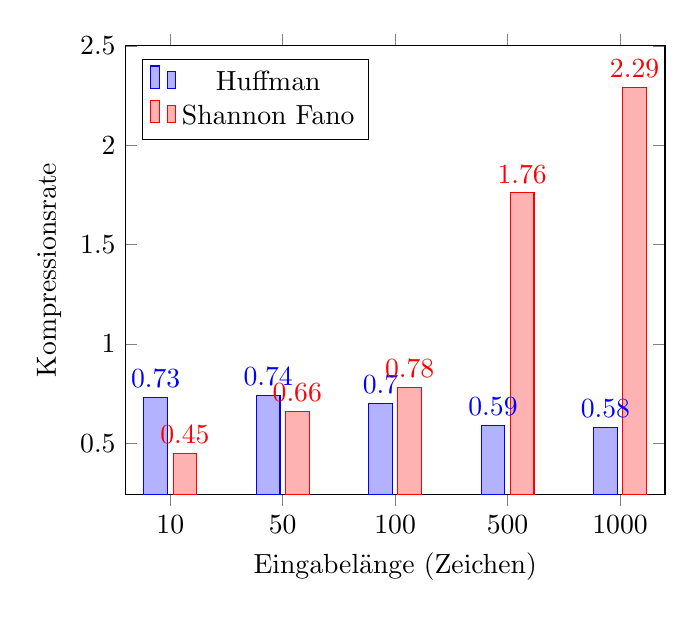
\begin{tikzpicture}
        \begin{axis}[
            legend pos=north west,
            bar width=0.3cm,
            ybar,
            ymax=2.5,
            symbolic x coords={10,50,100,500,1000},
            xtick=data,
            ylabel={Kompressionsrate},
            xlabel={Eingabelänge (Zeichen)},
            nodes near coords,
            nodes near coords align={vertical}]

        \addplot coordinates {(10,0.73) (50,0.74) (100,0.70) (500,0.59) (1000,0.58)};
        \addlegendentry{Huffman}
        \addplot coordinates {(10,0.45) (50,0.66) (100,0.78) (500,1.76) (1000,2.29)};
        \addlegendentry{Shannon Fano}

        \end{axis}
    \end{tikzpicture}
\end{center}
Die Tests spiegeln deutlich wieder, dass das Shannon-Fano Verfahrung für Eingaben bis zu einer Länge von 100 Zeichen im Allgemeinen eine bessere Kompressionsrate erbringt als die Huffman Kodierung. Jedoch ändert sich dies drastisch bei größeren Zeichenketten.\\
Erklärt werden kann dies durch die rekursive Verteilung der Codes. Wenn die Eingabehäufigkeit aller Buchstaben relativ gleichverteilt ist, wird bei Shannon-Fano öfters und gleichmäßiger rekursiv aufgeteilt was für jeden Code im Worst-Case $\log2(n)$ bedeutet. Anstatt sich die Häufigkeit zu Nutzen zu machen, wie es bei Huffman der Fall ist, wird (bei perfekter Aufteilung) ab einer Eingabe von 256 Zeichen die Kompressionsrate höher als eine direkte Abbildung der Zeichen auf Bitrepräsentation ($\log2(256)=8$).
%Quellencodierungssatz kommt stark: https://www.math.uni-frankfurt.de/~ismi/wakolbinger/teaching/StofI1819/1819Vorlesung15a.pdf%
\subsection{Optimierung}
Die Korrektheit des Huffman Codes war von Anfang an gegeben, jedoch haben wir durch einige Optimierungen die Zeit die unser Programm verbraucht hat reduzieren können. Die benutzten Optimierungen werden im Folgenden untersucht.\\\\
Gemessen wurde die Hauptimplementierung ohne jegliche Ein-/Ausgabe auf 10000 Durchläufen. Der "print dash" wurde nicht gesetzt was alle Konsolenausgaben ausgeschaltet. Es wurden 20 unterschiedliche \textit{Lorem ipsum} Teile %hier quelle rein
in Rotation bearbeitet mit unterschiedlicher Eingabelänge . Trotz meist lateinischer Wörter, stimmt die Verteilung der Häufigkeit der ausgewählten Text mit der der englischen als auch deutschen Sprache ausreichend überein um aussagefähige Resultate zu erhalten.

\begin{center}
    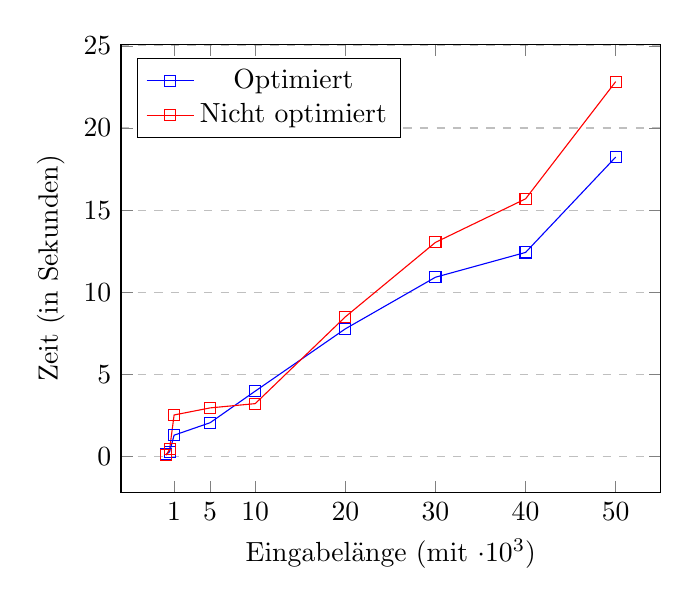
\begin{tikzpicture}
        \begin{axis}[
            xlabel={Eingabelänge (mit $\cdot 10^3$)},
            ylabel={Zeit (in Sekunden)},
            xtick={1,5,10,20,30,40,50},
            legend pos=north west,
            ymajorgrids=true,
            grid style=dashed,
            ]

        \addplot[
            color=blue,
            mark=square,
            ]
            coordinates {
            (0.1,0.14)(0.5,0.30)(1,1.31)(5,2.07)(10,3.99)(20,7.78)(30,10.92)(40,12.43)(50,18.23)
            };

        \addplot[
            color=red,
            mark=square,
            ]
            coordinates {
            (0.1,0.09)(0.5,0.45)(1,2.54)(5,2.97)(10,3.23)(20,8.51)(30,13.04)(40,15.69)(50,22.82)
            };

        \legend{Optimiert, Nicht optimiert}

        \end{axis}
    \end{tikzpicture}
\end{center}
Wie zu erwarten macht die Performanzmessungen schnell klar, dass die optimierte Version eine bessere Laufzeit hervorbringt. Im Allgemeinen hat die Optimierung erst eine Auswirkung auf Eingaben mit Längen ab 20000 Zeichen. Bei kleinen Eingaben macht es keinen großen Unterschied. Zudem scheint es, dass bei einem Versuch eine unglückliche Textkombination dazu geführt hat, dass die unoptimierte Version eine bessere Laufzeit darstellt. Dies ist jedoch im Allgemeinen nicht zu erwarten.\\
Analysiert man den Quellcode das Programmes stellt sich heraus, dass besonders das Zählen der Textlängen zu erheblichen Verlangsamungen geführt haben. Dies wurde oft mit der strlen(const char *s) Methode der string.h C-Bibliothek provoziert. Eine Lösung hierfür ist die Rückegabe der Daten, aber auch der Länge, nach dem Einlesen der Eingabe. Außerdem wird die Häufigkeit zuerst in einem Array der Länge 256 gezählt und erst im Anschluss die nicht leeren Häufigkeiten in einen Knoten tranformiert. Dies sorgt für schnelleren Zugriff und es müssen nur maximal 256 Knoten ohne weiteren Zugriff erstellt werden. Zu guter Letzt wurde in der optimierten Version die Kodierung der Buchstaben zuerst in eine Dictionary gespeichert und anschließend jeder Buchstaben einzeln kodiert. In der alten Version hat man dies entlang des Baumes gemacht was im schlimmsten Fall eine Laufzeit von log2(n) bedeutet. Beim Aufbauen des Dictionaries muss dies allerdings nur einmal getan werden.\\
Leider ist eine Optimierung hinsichtlich der Erstellung des Baumes nur schwierig möglich. Da immer die zwei kleinsten Häufigkeiten herausgenommen, zu einem Knoten verschmolzen und anschließend wieder hineingefügt werden. Daher ist es im Vorhinein unklar wo sich der neu zu erstellende Knoten befinden wird. Dies sorgt dafür, dass eine Laufzeit unter n * log2(n) nicht möglich ist.

\begin{center}
Die genannte Laufzeitanalyse wurde auf einem Apple MacBook Pro mit Silicon M1 Pro Chip, 16 GB Arbeitsspeicher und macOS Monterey 12.5.1 ausgeführt. Kompiliert wurde das Programm mit Apple clang version 14.0.0 (arm64-apple-darwin21.6.0) und der Option -O3.
\end{center}

\section{Zusammenfassung und Ausblick}

Insgesamt ist der Huffman Algorithmus, aufgrund seiner Optimalität bei symbolbasierter Komprimierung, immer noch sehr relevant, da er in den meisten Fällen sehr knapp an die, durch die Entropie gegebene, perfekte Komprimierung kommt.
Dennoch ist es möglich die Effizienz noch weiter zu erhöhen, indem man sich nicht nur auf symbolbasierte Algorithmen beschränkt.\\
Es wäre somit möglich, zum Beispiel bei von Menschen geschriebenen Fließtext, einen Huffman Baum für die einzelnen, durch Leerzeichen gentrennte, Wörter zu erstellen. Dies könnte bei sehr großen Quelldateien, im Vergleich zum symbolbasierten Ansatz, effizienter sein.\\
Eine spezielle Anpassung auf das gespeicherte Format sollte ebenfalls zu Optimierungen führen. Man denke sich, zum Beispiel, PNG für Bild- oder FLAC für Audiodateien, da hier mehr Daten, als nur Buchstaben, abgespeichert werden müssen.\\
Zu der Implementierung kann man sagen, dass diese noch deutlich optimierbar ist. Zu einem ist das Verfahren mit den Min-Heap sehr anschaulich, aber dafür ineffizient, da es auch Lösungswege gibt, die dies in $\mathcal{O}(n)$ erreichen \cite{Leeuwen1976OnTC}, unter anderem auch in-place \cite{10.1007/3-540-60220-8_79}.
Das Speicherformat könnte ebenfalls weiter optimiert werden, indem man, anstatt diese Menschenleslich zu strukturieren, direkt die Binärdaten reinschreibt. Zudem wäre es auch denkbar die Laufzeit, durch Parallelisierung und der Verwendung von mehreren Threads, zu reduzieren.\\
Zusammenfassend können wir sagen, das wir, durch das Projekt, zum optimierten Programmieren angeregt und somit ein hoher Lerneffekt erreicht wurde.

% TODO: Fuegen Sie Ihre Quellen der Datei Ausarbeitung.bib hinzu
% Referenzieren Sie diese dann mit \cite{}.
% Beispiel: CR2 ist ein Register der x86-Architektur~\cite{intel2017man}.
\bibliographystyle{plain}
\bibliography{Ausarbeitung}{}

\end{document}
